

  
  \frame{
  \frametitle{Dockerfile in a nutshell} 
  \begin{itemize}
  \item  Docker images can be built automatically by reading the instructions from a \textbf{\color{NavyBlue}Docker file};\vspace{0.2cm}
  \item  Docker file is a \textbf{\color{NavyBlue}simple text file} with the instructions on how to build your images;\vspace{0.2cm}
  \item The main Dockerfile commands are:\vspace{0.1cm}
  \begin{description}
  \item[FROM] It defines the base image to use  for the build process;
  \item[RUN]  It takes a command as its argument and runs it to form the image; 
  \item[COPY] It copies files from the source on the host into the container filesystem;
  \item[CMD]  It specifies what command to run within the container.  
  \end{description}
  \end{itemize}
  }
  
  
      \frame{
  \frametitle {Our first simple Docker image using dockerfile}
 This requires the following tasks:\vspace{0.4cm}
 \begin{itemize}
 \item Create a dockerfile;\vspace{0.2cm}	
 \item Create the images using the generated dockerfile.
 \end{itemize}
} 
  
        \frame{
  \frametitle {Our first simple Docker image using dockerfile}
 This requires the following tasks:\vspace{0.4cm}
 \begin{itemize}
 \item Create a dockerfile;\vspace{0.2cm}	\color{grey}
 \item Create the images using the generated dockerfile.
 \end{itemize}
} 
  
          \frame{
  \frametitle {Create a dockerfile}
  We use \textbf{\color{NavyBlue}gedit} to create our dockerfile; \vspace{0.2cm}
 \begin{center}
  			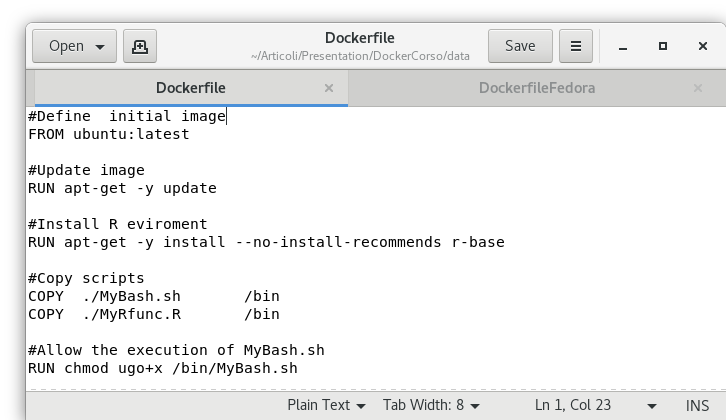
\includegraphics[width=0.93\columnwidth]{./Figure/gedit}
 \end{center} 
  }
   	  	
       \frame{
  \frametitle {Our first simple Docker image using dockerfile}
 This requires the following tasks:\vspace{0.4cm}
 \begin{itemize}
 \item Create a dockerfile;\vspace{0.2cm}	
 \item Create the images using the generated dockerfile.
 \end{itemize}
}   	  	


  	      \frame{
\frametitle{Building a Docker Image} 
  
 \emph{\color{PineGreen} docker build -t  $\langle \it{image} \rangle$ $\langle \it{path} \rangle$} can be used to build an image from a Dockerfile.
     	\begin{center}
  			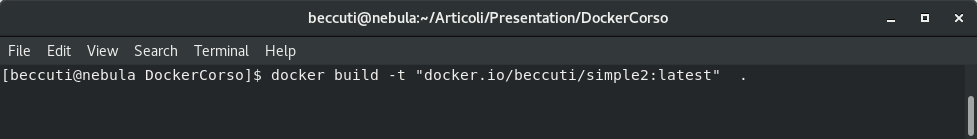
\includegraphics[width=1.00\columnwidth]{./Figure/build}
  		\end{center}  
  		     	\begin{center}
  			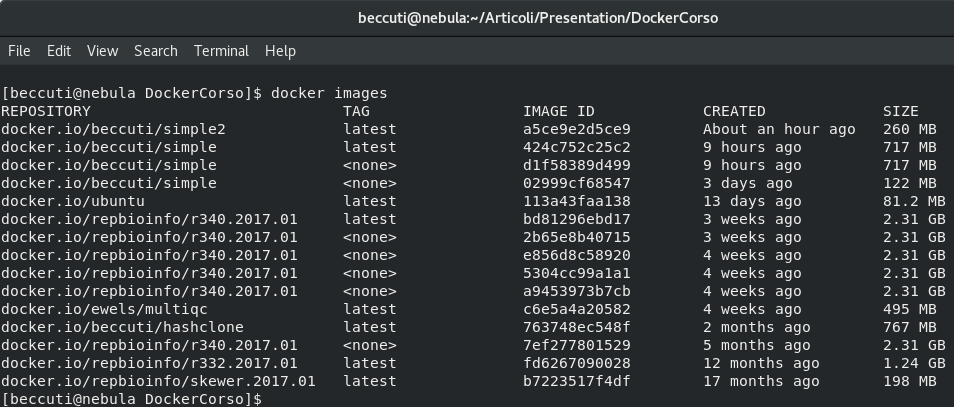
\includegraphics[width=1.00\columnwidth]{./Figure/build1}
  		\end{center}  
  
 }